
%{{第三十四回}}{第三十四回}}

\chapter{情中情因情感妹妹\\错里错以错劝哥哥}\label{part0038_split_000.htmlux5cux23calibre_pb_0}

{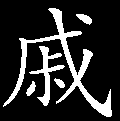
\includegraphics[width=3mm]{../Images/00005}两条素帕,一片真心;三首新诗,万行珠泪。袭卿高见动夫人,薛家兄妹空争气。自古道情是苦根苗,慧性灵心的,回头须早。}

话说袭人见贾母王夫人等去后,便走来宝玉身边坐下,含泪问他:``怎么就打到这步田地?''宝玉叹气说道:``不过为那些事,问他做什么!只是下半截疼的很,你瞧瞧打坏了那里。''袭人听说,便轻轻的伸手进去,将中衣褪下。宝玉略动一动,便咬着牙叫``嗳哟'',袭人连忙停住手,如此三四次才褪了下来。袭人看时,只见腿上半段青紫,都有四指宽的僵痕高了起来。袭人咬着牙说道:``我的娘,怎么下般的\href{../Text/part0038_split_000.html\#lnkback_1_a}{\textsuperscript{①}}这么狠手!你但凡听我一句话,也不得到这步地位。幸而没动筋骨,倘或打出个残疾来,可叫人怎么样呢!''

正说着,只听丫鬟们说:``宝姑娘来了。''袭人听见,知道穿不及中衣,便拿了一床袷纱被替宝玉盖了。只见宝钗手里托着一丸药走进来,{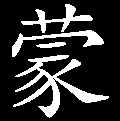
\includegraphics[width=3mm]{../Images/00006}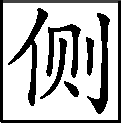
\includegraphics[width=3mm]{../Images/00011}\footnotesize \kaishu 请问是关心不是关心?}向袭人说道:``晚上把这药用酒研开,替他敷上,把那淤血的热毒散开,可以就好了。''说毕,递与袭人,又问道:``这会子可好些?''宝玉一面道谢说:``好了。''又让坐。宝钗见他睁开眼说话,不像先时,心中也宽慰了好些,便点头叹道:``早听人一句话,{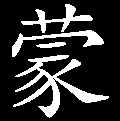
\includegraphics[width=3mm]{../Images/00006}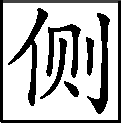
\includegraphics[width=3mm]{../Images/00011}\footnotesize \kaishu 同袭人语。}也不至今日。别说老太太、太太心疼,就是我们看着,心里也{(疼)}\ldots{}\ldots{}''\href{../Text/part0038_split_000.html\#lnkback_2_a}{\textsuperscript{②}}刚说了半句又忙咽住,自悔说的话急了,不觉的就红了脸,{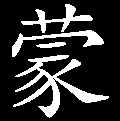
\includegraphics[width=3mm]{../Images/00006}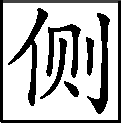
\includegraphics[width=3mm]{../Images/00011}\footnotesize \kaishu 行云流水语,微露半含时。}低下头来。宝玉听得这话如此亲切稠密,大有深意,忽见他又咽住不往下说,红了脸,低下头只管弄衣带,那一种娇羞怯怯,非可形容得出者,不觉心中大畅,将疼痛早丢在九霄云外,心中自思:``我不过捱了几下打,他们一个个就有这些怜惜悲感之态露出,令人可玩可观,可怜可敬。假若我一时竟遭殃横死,他们还不知是何等悲感呢!{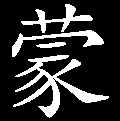
\includegraphics[width=3mm]{../Images/00006}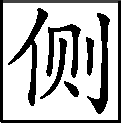
\includegraphics[width=3mm]{../Images/00011}\footnotesize \kaishu 得遇知己者,多生此等痴思痴喜。}既是他们这样,我便一时死了,得他们如此,一生事业纵然尽付东流,亦无足叹惜,冥冥之中若不怡然自得,亦可谓糊涂鬼祟矣。''想着,只听宝钗问袭人道:``怎么好好的动了气,就打起来了?''袭人便把茗烟的话说了出来。

宝玉原来还不知道贾环的话,见袭人说出方才知道。因又拉上薛蟠,惟恐宝钗沉心,忙又止住袭人道:``薛大哥哥从来不这样的,你们不可混猜度。''宝钗听说,便知道是怕他多心,用话相拦袭人,因心中暗暗想道:``打的这个形像,疼还顾不过来,还是这样细心,怕得罪了人,可见在我们身上也算是用心了。{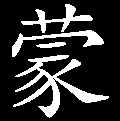
\includegraphics[width=3mm]{../Images/00006}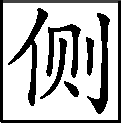
\includegraphics[width=3mm]{../Images/00011}\footnotesize \kaishu 天下古今英雄同一感慨。}你既这样用心,何不在外头大事上做工夫,老爷也欢喜了,也不能吃这样亏。但你固然怕我沉心,所以拦袭人的话,难道我就不知我的哥哥素日恣心纵欲,毫无防范的那种心性。当日为一个秦钟,还闹的天翻地覆,自然如今比先又更利害了。''想毕,因笑道:``你们也不必怨这个,怨那个。据我想,到底宝兄弟素日不正,肯和那些人来往,老爷才生气。就是我哥哥说话不防头,一时说出宝兄弟来,也不是有心调唆:一则也是本来的实话,二则他原不理论这些防嫌小事。袭姑娘从小儿只见宝兄弟这么样细心的人,{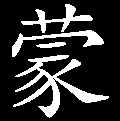
\includegraphics[width=3mm]{../Images/00006}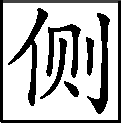
\includegraphics[width=3mm]{../Images/00011}\footnotesize \kaishu 心头口头不觉透漏。}你何尝见过天不怕地不怕、心里有什么口里就说什么的人。''

袭人因说出薛蟠来,见宝玉拦他的话,早已明白自己说造次了,恐宝钗没意思,听宝钗如此说,更觉羞愧无言。宝玉又听宝钗这番话,一半是堂皇正大,一半是去己疑心,更觉比先畅快了。方欲说话时,只见宝钗起身说道:``明儿再来看你,你好生养着罢。方才我拿了药来交给袭人,晚上敷上管就好了。''{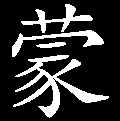
\includegraphics[width=3mm]{../Images/00006}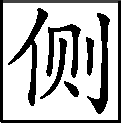
\includegraphics[width=3mm]{../Images/00011}\footnotesize \kaishu 何等关心!}说着便走出门去。袭人赶着送出院外,说:``姑娘倒费心了。改日宝二爷好了,亲自来谢。''宝钗回头笑道:``有什么谢处。你只劝他好生静养,别胡思乱想的就好了。{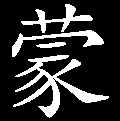
\includegraphics[width=3mm]{../Images/00006}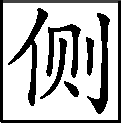
\includegraphics[width=3mm]{../Images/00011}\footnotesize \kaishu 的确真心。}要想什么吃的玩的,悄悄的往我那里去取了,不必惊动老太太、太太众人,倘或吹到老爷耳朵里,虽然彼时不怎么样,将来对景,终是要吃亏的。{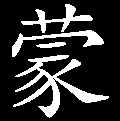
\includegraphics[width=3mm]{../Images/00006}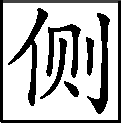
\includegraphics[width=3mm]{../Images/00011}\footnotesize \kaishu 要紧。}''说着,一面去了。

袭人抽身回来,心内着实感激宝钗。进来见宝玉沉思默默似睡非睡的模样,因而退出房外,自去栉沐。宝玉默默的躺在床上,无奈臀上作痛,如针挑刀挖一般,更又热如火炙,略展转时,禁不住``嗳哟''之声。那时天色将晚,因见袭人去了,却有两三个丫鬟伺候,此时并无呼唤之事,因说道:``你们且去梳洗,等我叫时再来。''众人听了,也都退出。

这里宝玉昏昏默默,只见蒋玉菡走了进来,诉说忠顺府拿他之事;又见金钏儿进来哭说为他投井之情。宝玉半梦半醒,都不在意。忽又觉有人推他,恍恍惚惚听得有人悲戚之声。宝玉从梦中惊醒,睁眼一看,不是别人,却是林黛玉。宝玉犹恐是梦,忙又将身子欠起来,向脸上细细一认,只见两个眼睛肿的桃儿一般,满面泪光,不是黛玉,却是那个?宝玉还欲看时,怎奈下半截疼痛难忍,支持不住,便``嗳哟''一声,仍就倒下,叹了一声,说道:``你又做什么跑来!虽说太阳落下去,那地上的馀热未散,走两趟又要受了暑。我虽然捱了打,并不觉疼痛。我这个样儿,只装出来哄他们,好在外头布散与老爷听,其实是假的。你不可认真。{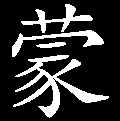
\includegraphics[width=3mm]{../Images/00006}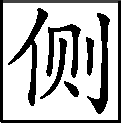
\includegraphics[width=3mm]{../Images/00011}\footnotesize \kaishu 有这样一段{(语)}{[}话{]},方不没灭颦儿之痛哭眼肿。英雄失足,每每至死不改,皆犹此耳。}''此时林黛玉虽不是嚎啕大哭,然越是这等无声之泣,气噎喉堵,更觉得利害。听了宝玉这番话,心中虽然有万句言词,只是不能说得,半日,方抽抽噎噎的说道:``你从此可都改了罢!''{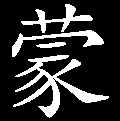
\includegraphics[width=3mm]{../Images/00006}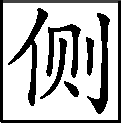
\includegraphics[width=3mm]{../Images/00011}\footnotesize \kaishu 心血淋漓,酿成此数字。}宝玉听说,便长叹一声,道:``你放心,别说这样话。就便为这些人死了,{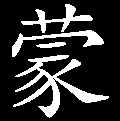
\includegraphics[width=3mm]{../Images/00006}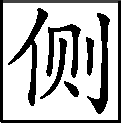
\includegraphics[width=3mm]{../Images/00011}\footnotesize \kaishu 文气斩截。}也是情愿的!''一句话未了,只见院外人说:``二奶奶来了。''林黛玉便知是凤姐来了,连忙立起身说道:``我从后院子去罢,回来再来。''宝玉一把拉住道:``这可奇了,好好的怎么怕起他来。''林黛玉急的跺脚,悄悄的说道:``你瞧瞧我的眼睛,又该他取笑开心呢。''{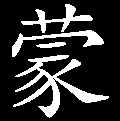
\includegraphics[width=3mm]{../Images/00006}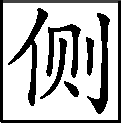
\includegraphics[width=3mm]{../Images/00011}\footnotesize \kaishu 不避嫌疑,不惜声名,破格牵连,诚为可叹,着实可怜。}宝玉听说,赶忙的放手。黛玉三步两步转过床后,出后院而去。凤姐从前头已进来了,问宝玉:``可好些了?想什么吃,叫人往我那里取去。''接着,薛姨妈又来了。一时贾母又打发了人来。

至掌灯时分,宝玉只喝了两口汤,便昏昏沉沉的睡去。接着,周瑞媳妇、吴新登媳妇、郑好时媳妇这几个有年纪常往来的,听见宝玉捱了打,也都进来。袭人忙迎出来,悄悄的笑道:``婶婶们来迟了一步,{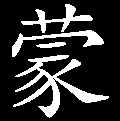
\includegraphics[width=3mm]{../Images/00006}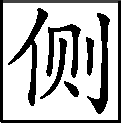
\includegraphics[width=3mm]{../Images/00011}\footnotesize \kaishu 袭卿善词令,会周旋。}二爷才睡着了。''说着,一面带他们到那边房里坐了,倒茶与他们吃。那几个媳妇子都悄悄的坐了一回,向袭人说:``等二爷醒了,你替我们说罢。''

袭人答应了,送他们出去。刚要回来,只见王夫人使个婆子来,口称``太太叫一个跟二爷的人呢''。袭人见说,想了一想,便回身悄悄告诉晴雯、麝月、檀云、秋纹等说:``太太叫人,你们好生在房里,我去了就来。''{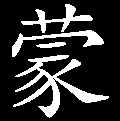
\includegraphics[width=3mm]{../Images/00006}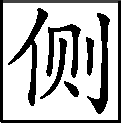
\includegraphics[width=3mm]{../Images/00011}\footnotesize \kaishu 身任其责,不惮劳烦。}说毕,同那婆子一径出了园子,来至上房。王夫人正坐在凉榻上摇着芭蕉扇子,见他来了,说:``不管叫个谁来也罢了。你又丢下他来了,谁伏侍他呢?''袭人见说,连忙陪笑回道:``二爷才睡安稳了,那四五个丫头如今也好了,会伏侍二爷了,太太请放心。恐怕太太有什么话吩咐,打发他们来,一时听不明白,倒耽误了。''{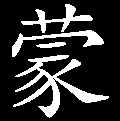
\includegraphics[width=3mm]{../Images/00006}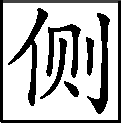
\includegraphics[width=3mm]{../Images/00011}\footnotesize \kaishu 能事解事,能了事。}王夫人道:``也没甚话,白问问他这会子疼的怎么样。''袭人道:``宝姑娘送去的药,我给二爷敷上了,{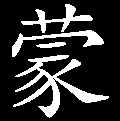
\includegraphics[width=3mm]{../Images/00006}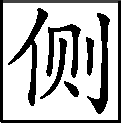
\includegraphics[width=3mm]{../Images/00011}\footnotesize \kaishu 补足。}比先好些了。先疼的躺不稳,这会子都睡沉了,可见好些了。''王夫人又问:``吃了什么没有?''袭人道:``老太太给的一碗汤,喝了两口,只嚷干渴,要吃酸梅汤。我想着酸梅是个收敛的东西,才刚捱了打,又不许叫喊,自然急的那热毒热血未免不存在心里,倘或吃下这个去激在心里,再弄出大病来,可怎么样呢。因此我劝了半天才没吃,{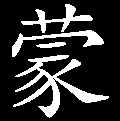
\includegraphics[width=3mm]{../Images/00006}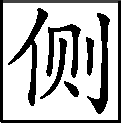
\includegraphics[width=3mm]{../Images/00011}\footnotesize \kaishu 能事处。}只拿那糖腌的玫瑰卤子和了吃,吃了半碗,又嫌吃絮了,不香甜。''王夫人道:``嗳哟,你不该早来和我说。前儿有人送了两瓶子香露来,原要给他点子的,我怕他胡糟踏了,就没给。既是他嫌那些玫瑰膏子絮烦,把这个拿两瓶子去。一碗水里只用挑一茶匙儿,就香的了不得呢。''说着就唤彩云来,``把前儿的那几瓶香露拿了来。''袭人道:``只拿两瓶来罢,多了也白糟踏。等不够再要,再来取也是一样。''彩云听说,去了半日,果然拿了两瓶来,付与袭人。袭人看时,只见两个玻璃小瓶,却有三寸大小,上面螺丝银盖,鹅黄笺上写着``木樨清露'',那一个写着``玫瑰清露''。袭人笑道:``好金贵东西!这么个小瓶儿,能有多少?''王夫人道:``那是进上的,你没看见鹅黄笺子?你好生替他收着,别糟踏了。''

袭人答应着,方要走时,王夫人又叫:``站着,我想起一句话来问你。''袭人忙又回来。王夫人见房内无人,便问道:``我恍惚听见宝玉今儿捱打,是环儿在老爷跟前说了什么话。你可听见这个了?你要听见,告诉我听听,我也不吵出来教人知道是你说的。''袭人道:``我倒没听见这话,为二爷霸占着戏子,人家来和老爷要,为这个打的。''王夫人摇头说道:``也为这个,还有别的原故。''袭人道:``别的原故实在不知道了。我今儿在太太跟前大胆说句不知好歹的话。论理\ldots{}\ldots{}''说了半截忙又咽住。王夫人道:``你只管说。''袭人笑道:``太太别生气,我就说了。''王夫人道:``我有什么生气的,你只管说来。''

袭人道:``论理,我们二爷也须得老爷教训两顿。若老爷再不管,将来不知做出什么事来呢。''王夫人一闻此言,便合掌念声``阿弥陀佛'',{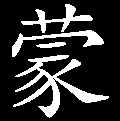
\includegraphics[width=3mm]{../Images/00006}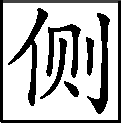
\includegraphics[width=3mm]{../Images/00011}\footnotesize \kaishu 能了事处。}由不得赶着袭人叫了一声``我的儿,亏了你也明白,这话和我的心一样。{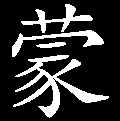
\includegraphics[width=3mm]{../Images/00006}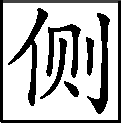
\includegraphics[width=3mm]{../Images/00011}\footnotesize \kaishu 袭卿之心,所谓``良人所仰望而终身也''。今若此,能不痛哭流{(泣)}{[}涕{]},以成此语?}我何曾不知道管儿子,先时你珠大爷在,我是怎么样管他,难道我如今倒不知管儿子了?只是有个原故:如今我想,我已经快五十岁的人,通共剩了他一个,他又长的单弱,况且老太太宝贝似的,若管紧了他,倘或再有个好歹,或是老太太气坏了,那时上下不安,岂不倒坏了,所以就纵坏了他。我常常掰着口儿劝一阵,说一阵,气的骂一阵,哭一阵,彼时他好,过后儿还是不相干,端的吃了亏才罢了。若打坏了,将来我靠谁呢!''{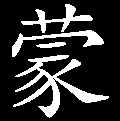
\includegraphics[width=3mm]{../Images/00006}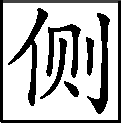
\includegraphics[width=3mm]{../Images/00011}\footnotesize \kaishu 变转之句,勉强之言,真体贴尽溺爱之心。}说着,由不得滚下泪来。

袭人见王夫人这般悲感,自己也不觉伤了心,陪着落泪。又道:``二爷是太太养的,岂不心疼。便是我们做下人的伏侍一场,大家落个平安,也算是造化了。要这样起来,连平安都不能了。那一日那一时我不劝二爷,只是再劝不醒。偏生那些人又肯亲近他,也怨不得他这样,总是我们劝的倒不好了。今儿太太提起这话来,我还记挂着一件事,每要来回太太,讨太太个主意。只是我怕太太疑心,不但我的话白说了,且连葬身之地都没了。''{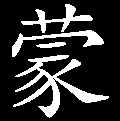
\includegraphics[width=3mm]{../Images/00006}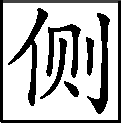
\includegraphics[width=3mm]{../Images/00011}\footnotesize \kaishu 打进一层。非有前项如许讲究,这一层即为唐突了。}王夫人听了这话内有因,忙问道:``我的儿,你有话只管说。近来我因听见众人背前背后都夸你,我只说你不过是在宝玉身上留心,或是诸人跟前和气,这些小意思好,所以将你和老姨娘一体行事。谁知你方才和我说的话全是大道理,正和我的想头一样。你有什么只管说什么,只别教别人知道就是了。''

袭人道:``我也没什么别的说。我只想着讨太太一个示下,怎么变个法儿,以后竟还教二爷搬出园外来就好了。''王夫人听了,吃一大惊,忙拉了袭人的手问道:``宝玉难道和谁作怪了不成?''袭人忙回道:``太太别多心,并没有这话。这不过是我的小见识。如今二爷也大了,里头姑娘们也大了,况且林姑娘宝姑娘又是两姨姑表姊妹,虽说是姊妹们,到底是男女之分,日夜一处起坐不方便,由不得叫人悬心,{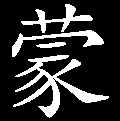
\includegraphics[width=3mm]{../Images/00006}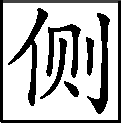
\includegraphics[width=3mm]{../Images/00011}\footnotesize \kaishu 远忧近虑,言言字字,真是可人。}便是外人看着也不像。一家子的事,俗语说的`没事常思有事',世上多少无头脑的事,多半因为无心中做出,有心人看见,当做有心事,反说坏了。只是预先不防着,断然不好。二爷素日性格,太太是知道的。他又偏好在我们队里闹,倘或不防,前后错了一点半点,不论真假,人多口杂,那起小人的嘴有什么避讳,心顺了,说的比菩萨还好,心不顺,就贬的连畜牲不如。二爷将来倘或有人说好,不过大家直过没事;若叫人说出一个不好字来,我们不用说,粉身碎骨,罪有万重,都是平常小事,但后来二爷一生的声名品行岂不完了,{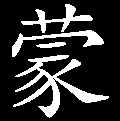
\includegraphics[width=3mm]{../Images/00006}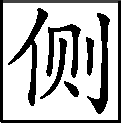
\includegraphics[width=3mm]{../Images/00011}\footnotesize \kaishu 袭卿爱人以德,竟至如此。字字逼来,不觉令人敬听。看官自省,切{[}不{]}可阔略,戒之。}二则太太也难见老爷。俗语又说`君子防不然',不如这会子防避的为是。太太事情多,一时固然想不到。我们想不到则可,既想到了,若不回明太太,罪越重了。近来我为这事日夜悬心,又不好说与人,惟有灯知道罢了。''

王夫人听了这话,如雷轰电掣一般,正触了金钏儿之事,心内越发感爱袭人不尽,忙笑道:``我的儿,你竟有这个心胸,想的这样周全!我何曾又不想到这里,只是这几次有事就忘了。你今儿这一番话提醒了我。难为你成全我娘儿两个声名体面,真真我竟不知道你这样好。罢了,你且去罢,我自有道理。{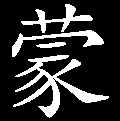
\includegraphics[width=3mm]{../Images/00006}\includegraphics[width=3mm]{../Images/00011}\footnotesize \kaishu 溺爱者偏会如此说。}只是还有一句话:你如今既说了这样的话,我就把他交给你了,好歹留心,保全了他,就是保全了我。我自然不辜负你。''

袭人连连答应着去了。回来正值宝玉睡醒,袭人回明香露之事。宝玉喜不自禁,即令调来尝试,果然香妙非常。因心下记挂着黛玉,满心里要打发人去,只是怕袭人,便设一法,先使袭人往宝钗那里去借书。

袭人去了,宝玉便悄命晴雯{\includegraphics[width=3mm]{../Images/00003}\includegraphics[width=3mm]{../Images/00012}\footnotesize \kaishu 前文晴雯放肆,原有把柄所持也。}吩咐道:``你到林姑娘那里看看他做什么呢。他要问我,只说我好了。''晴雯道:``白眉赤眼,做什么去呢?到底说句话儿,也像一件事。''宝玉道:``没有什么可说的。''晴雯道:``若不然,或是送件东西,或是取件东西,不然我去了怎么搭讪呢?''宝玉想了一想,便伸手拿了两条手帕子撂与晴雯,笑道:``也罢,就说我叫你送这个给他去了。''晴雯道:``这又奇了。他要这半新不旧的两条手帕子?他又要恼了,说你打趣他。''宝玉笑道:``你放心,他自然知道。''

晴雯听了,只得拿了帕子往潇湘馆来。只见春纤正在栏杆上晾手帕子,{\includegraphics[width=3mm]{../Images/00006}\includegraphics[width=3mm]{../Images/00011}\footnotesize \kaishu 送的是手帕,晾的是手帕,妙文。}见他进来,忙摆手儿,说:``睡下了。''晴雯走进来,满屋魆黑,并未点灯。黛玉已睡在床上,问是谁。晴雯忙答道:``晴雯。''黛玉道:``做什么?''晴雯道:``二爷送手帕子来给姑娘。''黛玉听了,心中发闷:``做什么送手帕子来给我?''因问:``这帕子是谁送他的?必是上好的,叫他留着送别人罢,我这会子不用这个。''晴雯笑道:``不是新的,就是家常旧的。''林黛玉听见,越发闷住,着实细心搜求,思忖一时,方大悟过来,连忙说:``放下,去罢。''晴雯听了,只得放下,抽身回去,一路盘算,不解何意。

这里林黛玉体贴出手帕子的意思来,不觉神魂驰荡:宝玉这番苦心,能领会我这番苦意,又令我可喜;我这番苦意,不知将来如何,又令我可悲;忽然好好的送两块旧帕子来,若不是领我深意,单看了这帕子,又令我可笑;再想令人私相传递与我,又可惧;我自己每每好哭,想来也无味,又令我可愧。如此左思右想,一时五内沸然炙起。黛玉由不得馀意绵缠,令掌灯,也想不起嫌疑避讳等事,便向案上研墨蘸笔,便向那两块旧帕上走笔写道:

眼空蓄泪泪空垂,暗洒闲抛却为谁?

尺幅鲛鮹劳解赠,叫人焉得不伤悲!

其二

抛珠滚玉只偷潸,镇日无心镇日闲;

枕上袖边难拂拭,任他点点与斑斑。

其三

彩线难收面上珠,湘江旧迹已模糊;

窗前亦有千竿竹,不识香痕渍也无?

林黛玉还要往下写时,觉得浑身火热,面上作烧,走至镜台揭起锦袱一照,只见腮上通红,自羡压倒桃花,却不知病由此萌。一时方上床睡去,犹拿着那帕子思索,不在话下。

却说袭人来见宝钗,谁知宝钗不在园内,往他母亲那里去了,袭人便空手回来。等至二更,宝钗方回来。原来宝钗素知薛蟠情性,心中已有一半疑是薛蟠调唆了人来告宝玉的,谁知又听袭人说出来,越发信了。究竟袭人是听茗烟说的,那茗烟也是私心窥度,并未据实,竟认准是他说的。那薛蟠都因素日有这个名声,其实这一次却不是他干的,被人生生的一口咬死是他,有口难分。这日正从外头吃了酒回来,见过母亲,只见宝钗在这里,说了几句闲话,因问:``听见宝兄弟吃了亏,是为什么?''薛姨妈正为这个不自在,见他问时,便咬着牙道:``不知好歹的东西,都是你闹的,你还有脸来问!''薛蟠见说,便怔了,忙问道:``我何尝闹什么?''薛姨妈道:``你还装憨呢!人人都知道是你说的,还赖呢。''薛蟠道:``人人说我杀了人,也就信了罢?''薛姨妈道:``连你妹妹都知道是你说的,难道他也赖你不成?''宝钗忙劝道:``妈和哥哥且别叫喊,消消停停的,就有个青红皂白了。''因向薛蟠道:``是你说的也罢,不是你说的也罢,事情也过去了,不必较证,倒把小事儿弄大了。我只劝你从此以后在外头少去胡闹,少管别人的事。天天一处大家胡逛,你是个不防头的人,过后儿没事就罢了,倘或有事,不是你干的,人人都也疑惑是你干的,不用说别人,我就先疑惑。''

薛蟠本是个心直口快的人,一生见不得这样藏头露尾的事,又见宝钗劝他不要逛去,他母亲又说他犯舌,宝玉之打是他治的,早已急的乱跳,赌身发誓的分辩。又骂众人:``谁这样赃派我?我把那囚攮的牙敲了才罢!分明是为打了宝玉,没的献勤儿,拿我来作幌子。难道宝玉是天王?他父亲打他一顿,一家子定要闹几天。那一回为他不好,姨爹打了他两下子,过后老太太不知怎么知道了,说是珍大哥哥治的,好好的叫了去骂了一顿。今儿越发拉上我了!既拉上,我也不怕,越性进去把宝玉打死了,我替他偿了命,大家干净。''一面嚷,一面抓起一根门闩来就跑。慌的薛姨妈一把抓住,骂道:``作死的孽障,你打谁去?你先打我来!''

薛蟠急的眼似铜铃一般,嚷道:``何苦来!又不叫我去,又好好的赖我。将来宝玉活一日,我担一日的口舌,不如大家死了清净。''宝钗忙也上前劝道:``你忍耐些儿罢。妈急的这个样儿,你不说来劝妈,你还反闹的这样。别说是妈,便是旁人来劝你,也为你好,倒把你的性子劝上来了。''薛蟠道:``这会子又说这话。都是你说的!''宝钗道:``你只怨我说,再不怨你顾前不顾后的形景。''薛蟠道:``你只会怨我顾前不顾后,你怎么不怨宝玉外头招风惹草的那个样子!别说多的,只拿前儿琪官的事比给你们听:那琪官,我们见过十来次的,我并未和他说一句亲热话;怎么前儿他见了,连姓名还不知道,就把汗巾子给他了?难道这也是我说的不成?''薛姨妈和宝钗急的说道:``还提这个!可不是为这个打他呢。可见是你说的了。''薛蟠道:``真真的气死了人了!赖我说的我不恼,我只为一个宝玉闹的这么天翻地覆的。''宝钗道:``谁闹了?你先持刀动杖的闹起来,倒说别人闹。''

薛蟠见宝钗说的句句有理,难以驳正,比母亲的话反难回答,因此便要设法拿话堵回他去,就无人敢拦自己的话了;也因正在气头儿上,未曾想话之轻重,便说道:``好妹妹,你不用和我闹,我早知道你的心了。从先妈和我说,你这金要拣有玉的才可正配,你留了心,见宝玉有那劳什骨子,你自然如今行动护着他。''话未说了,把个宝钗气怔了,拉着薛姨妈哭道:``妈妈你听,哥哥说的是什么话!''{\includegraphics[width=3mm]{../Images/00006}\includegraphics[width=3mm]{../Images/00011}\footnotesize \kaishu 插写薛蟠,不过要补足宝钗告袭人前项之言。}薛蟠见妹妹哭了,便知自己冒撞了,便赌气走到自己房里安歇不提。

这里薛姨妈气的乱战,一面又劝宝钗道:``你素日知那孽障说话没道理,明儿我叫他给你陪不是。''宝钗满心委屈气忿,待要怎样,又怕他母亲不安,少不得含泪别了母亲,各自回来,到房里整哭了一夜。次日早起来,也无心梳洗,胡乱整理整理,便出来瞧母亲。可巧遇见林黛玉独立在花阴之下,问他那里去。薛宝钗因说``家去'',口里说着,便只管走。黛玉见他无精打采的去了,又见眼上有哭泣之状,大非往日可比,便在后面笑道:``姐姐也自保重些儿。就是哭出两缸眼泪来,也医不好棒疮!''{\includegraphics[width=3mm]{../Images/00006}\includegraphics[width=3mm]{../Images/00011}\footnotesize \kaishu 自己眼肿为谁?偏是以此笑人。世间人多犯此症。}不知宝钗如何答对,且听下回分解。

{\includegraphics[width=3mm]{../Images/00005}总评:人有百折不回之真心,方能成旷世稀有之事业。宝玉意中诸多辐辏,所谓``求仁得仁,又何怨?''凡人作臣作子,出入家庭廊庙,能推此心此志,何患忠孝之不全、事业之不立耶?}

{\href{../Text/part0038_split_000.html\#navto_1_a}{①}``怎么下般的这么狠手'',己本同。蒙、戚、辰本作``怎么下这般的狠手'',列、杨本作``怎么下的这么毒手'',当系不知``下般''词义而擅改。按:下般,犹忍心。《金瓶梅词话》第二六回:``月娘见他吓得那等腔儿,心中又下般不的。此时你恁害怕,当初大家省言一句儿便了。''同书第七五回:``紧教人疼的魂也没了,还要那等掇弄人,亏你也下般的。''}

{\href{../Text/part0038_split_000.html\#navto_2_a}{②}按:此句完整,不像``说了半句'',各本均同,唯己卯本点去``心里也疼''四字。程本作``心里也''。}
